\chapter{Introdução} \label{sch:intro}
Nesse capítulo será apresentado uma pouco da história a computação moderna e do
contexto histórico no qual o TeX e o LaTeX surgiram. Posteriormente encontra-se
um glossário de termos relacionados com o LaTeX.

\section{História}
Podemos dizer que a história da computação moderna tem início com a criação do
ENIAC (Electronic Numerical Integrator and Computer), o primeiro computador
digital eletrônico de grande escala, criado em fevereiro de 1946 pelos
cientistas norte-americanos John Eckert e John Mauchly, da Electronic Control
Company.\nocite{Wikipedia:PT:ENIAC}

Por muitos anos o uso de computadores ficou restrito a grandes empresas e
universidades como AT\&T Bell Labs, General Electric, Massachusetts Institute of
Technology entre outros. Em 1969 foi lançado o sistema operacional UNIX que
rapidamente passou a ser utilizado pela maioria dos usuários da
época.\nocite{Wikipedia:EN:UNIX}

Nos anos 70 ocorreu uma grande mudança nas técnicas de produção de livros e
similares. Em 1977, Donald Knuth lançou a segunda edição do segundo volume de
sua obra ``The Art of Computer Programming'' e não gostou do resultado (na
primeira edição havia sido utilizada uma técnica de impressão diferente). Por
volta desse ano, Knuth viu pela primeira vez o resultado de um sistema
tipográfico digital de alta qualidade e ficou interessado pelo mesmo. Motivado
pelo ``problema'' com o seu livro ele acabou desenvolvendo o seu próprio sistema
tipográfico, o TeX\footnote{A pronúncia correta é semelhante a da palavra
inglesa ``tech''. Maiores informações em
\url{http://www.tex.ac.uk/cgi-bin/texfaq2html?label=TeXpronounce}}, que foi
lançado em 1978.\nocite{Wikipedia:EN:TeX}

Usar o TeX não era fácil. Em 1985, Leslie Lamport lança o LaTeX, uma linguagem
de marcação e preparativo do sistema para o TeX, facilitando a utilização do
TeX.\nocite{Wikipedia:EN:LaTeX}

Os primeiros computadores pessoais, como o Apple I, surgem nos anos 70. E nos
anos 80 os computadores começam a invadir escritórios e depois lares, sendo que
nessa década são lançados o IBM Personal Computer (IBM PC), Lisa, Macintosh e
vários clones (principalmente do IBM PC).

Em 1985, uma pequena \textit{start-up} chamada Microsoft lança seu sistema
operacional, Windows, e seu processador de texto, Word, que possuia uma versão
para Macintosh e foi um dos primeiros a possuir funcionalidades verdadeiramente
WYSIWYG\footnote{Acrônimo da expressão em inglês ``What You See Is What You
Get'', cuja tradução remete a algo como ``O que você vê é o que você obtem''.}.
Por ser WYSIWYG,  utilizar o Word ou algum de seus concorrentes não exigia
nenhum conhecimento prévio e isso acabou ofuscando o LaTeX.\footnote{É
importante destacar que, tipicamente, os usuários do LaTeX (ou TeX) e do Word
(ou concorrêntes) possuem necessidades bastante diferentes.}

Com os computadores pessoais a Microsoft acabou adquirindo grande parte do
mercado de sistemas operacionais para o seu produto, o Windows, por este ser
compatível com os clones do IBM PC e possuir interface gráfica.\footnote{Nessa
época a Apple ainda era uma \textit{start-up} quando comparada a seus
concorrentes como, por exemplo, a IBM e ocorria a \textit{UNIX wars} (ver
detalhes em \url{http://en.wikipedia.org/wiki/Unix_wars}).} Desde que o Windows
passou a ser o sistema operacional dominante\footnote{Ao menos no ramo de
computadores pessoais.} a Microsoft violou várias leis antitruste para promover
outros de seus produtos como seu pacote de escritório, Microsoft Office, que
inclue o Word, seu navegador de internet, Internet Explorer, e outros.

\begin{figure}[htb]
  \begin{center}
    % Filename: history_timeline1@latex_with_vim.tex
% This code is part of LaTeX with Vim.
% 
% Description: TikZ for teachers is free book about TikZ and Sage.
% 
% Created: 30.03.12 07:55:25 PM
% Last Change: 30.03.12 07:56:41 PM
% 
% Author: Raniere Gaia Costa da Silva, r.gaia.cs@gmail.com
% Organization:  
% 
% Copyright (c) 2010, 2011, 2012, Raniere Gaia Costa da Silva. All rights 
% reserved.
% 
% This file is license under the terms of a Creative Commons Attribution 
% 3.0 Unported License, or (at your option) any later version. More details
% at <http://creativecommons.org/licenses/by/3.0/>.
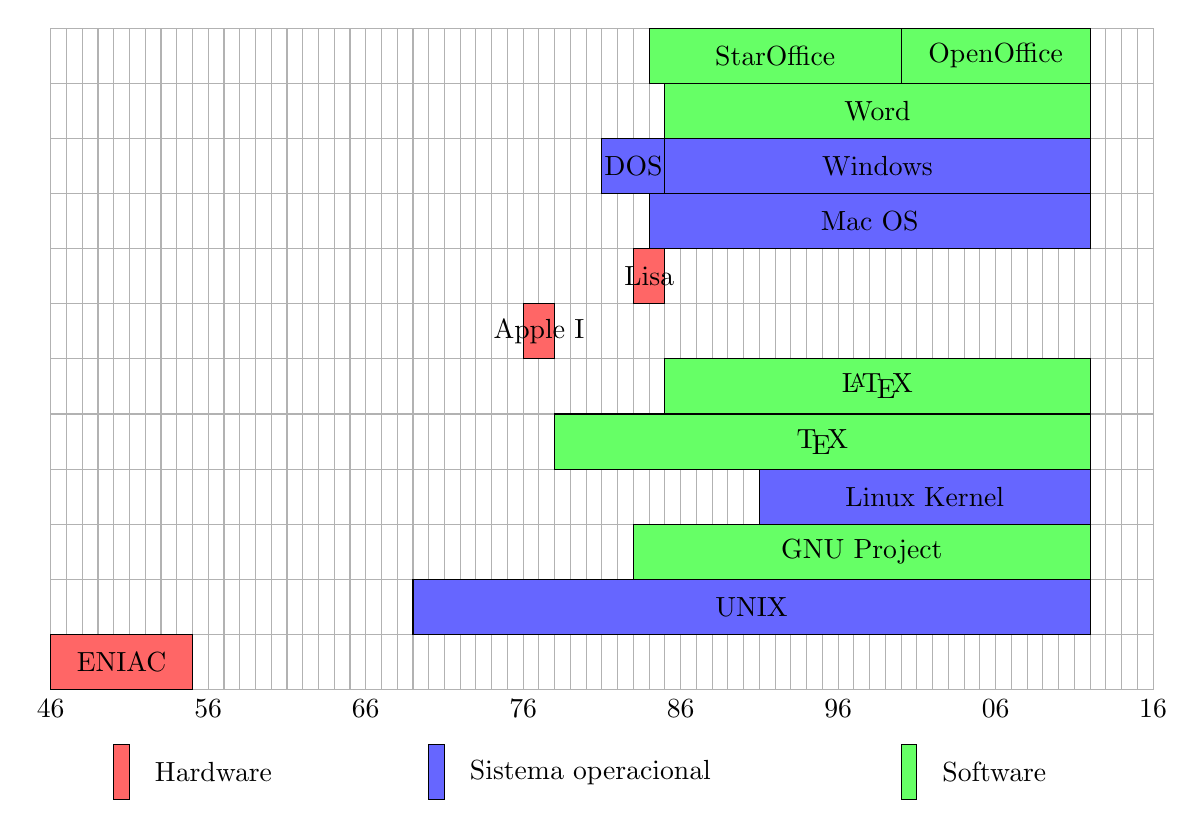
\begin{tikzpicture}[xscale=0.2, yscale=0.7]
    \draw[gray!60] (46,0) grid (116,12);
    \foreach \y in {46, 56, ..., 96}{
        \node[below] at (\y, 0) {\y};
    }
    \node[below] at (106,0) {06};
    \node[below] at (116,0) {16};

    \draw[fill=red!60] (50,-1) rectangle ++(1,-1) ++(1,.5) node[right]{Hardware};
    \draw[fill=blue!60] (70,-1) rectangle ++(1,-1) ++(1,.5) node[right]{Sistema operacional};
    \draw[fill=green!60] (100,-1) rectangle ++(1,-1) ++(1,.5) node[right]{Software};

    \draw[fill=red!60] (46,0) rectangle (55,1) node[midway]{ENIAC};
    \draw[fill=blue!60] (69,1) rectangle (112,2) node[midway]{UNIX};
    \draw[fill=green!60] (83,2) rectangle (112,3) node[midway]{GNU Project};
    \draw[fill=blue!60] (91,3) rectangle (112,4) node[midway]{Linux Kernel};
    \draw[fill=green!60] (78,4) rectangle (112,5) node[midway]{\TeX};
    \draw[fill=green!60] (85,5) rectangle (112,6) node[midway]{\LaTeX};
    \draw[fill=red!60] (76,6) rectangle (78,7) node[midway]{Apple I};
    \draw[fill=red!60] (83,7) rectangle (85,8) node[midway]{Lisa};
    \draw[fill=blue!60] (84,8) rectangle (112,9) node[midway]{Mac OS};
    \draw[fill=blue!60] (81,9) rectangle (85,10) node[midway]{DOS};
    \draw[fill=blue!60] (85,9) rectangle (112,10) node[midway]{Windows};
    \draw[fill=green!60] (85,10) rectangle (112,11) node[midway]{Word};
    \draw[fill=green!60] (84,11) rectangle (100,12) node[midway]{StarOffice};
    \draw[fill=green!60] (100,11) rectangle (112,12) node[midway]{OpenOffice};
\end{tikzpicture}

  \end{center}
  \caption{Linha do tempo de alguns softwares.}
  \label{fig:history_timeline}
\end{figure}

\section{Glossário}
Ao procurar ajuda é fundamental utilizar a palavra correta para o que deseja-se
e como existem várias palavras que incluem TeX espera-se ajudar o leitor com
algumas explicações (em ordem alfabética):
\begin{description}
  \item[compilador] é o arquivo binário responsável por ler o arquivo
    \lstinline+.tex+ e criar o arquivo para impressão.
  \item[distribuição] uma coleção estruturada de software relacionados.
    Alguns exemplos de destribuições (La)TeX são: TeX Live e MiKTeX.
  \item[dvi] acrônimo para DeVice-Independent.
  \item[LaTeX] é o conjunto de macros escrita por Lamport para o TeX.
  \item[pdf] acrônimo para Portable Document Format.
  \item[ps] ou PostScript é linguagem para criação de desenhos vetoriais.
  \item[TeX] é o sistema tipográfico criado por Knuth.
\end{description}
